\subsection{Структурно функциональная схема программного обеспечения}%, в состав которого входит разрабатываемый программный модуль с четкой формулировкой решаемых им задач}

Программное обеспечение состоит из нескольких блоков, представленных на рисунке \ref{pic:shema_PO}.

\begin{itemize}
\item ПО для оценки деформации ``Deformation Analysis''
\item Форма для ввода входных параметров ``strain\_calculate.qml''
\item ПО для расчёта деформации твердого тела ``lucas\_kanade''
\end{itemize}

Программа ``Deformation Analysis'' разрабатывалась сотрудниками ИФПМ и служит средством для запуска и отображения выходных результатов. Форма ``strain\_calculate.qml'' является более удобным способом запуска основного приложения. 

\begin{figure}[ht]
\center{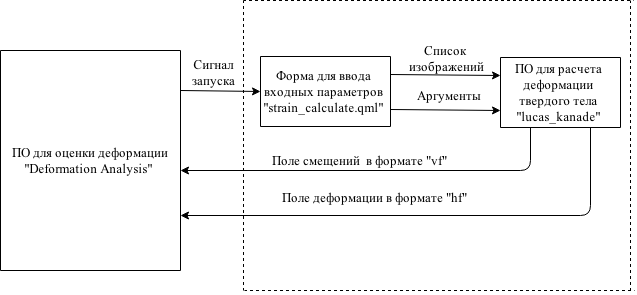
\includegraphics[width=0.8\linewidth]{shema_PO}}
\caption{Структура разработанного ПО}
\label{pic:shema_PO}
\end{figure}

\begin{figure}[ht]
\center{
\includegraphics[width=0.8\linewidth]{idef0}}
\caption{Функциональная схема}
\label{pic:idef0}
\end{figure}

\subsection{Характеристику входных и выходных информационных потоков разрабатываемого модуля}
Для корректной работы разрабатываемого программного комплекса, компьютер должен отвечать следующим требованиям:
\subsubsection {Минимальные требования к аппаратному обеспечению}
Минимальные системные требования для операционной системы Linux Debian 8~\cite{debian_8}:

\begin{itemize}
\item процессор 1ГГц Pentium 4;
\item оперативная память 512 Мб;
\item место на жёстком диске -- 9 Гб.
\end{itemize}

Минимальные системные требования для операционной системы Microsoft Windows 7~\cite{windows_7}:

\begin{itemize}
\item процессор 32-разрядный или 64-разрядный 1 ГГц;
\item оперативная память 1 Гб для 32-разрядной системы или 2 Гб для 64-разрядной системы;
\item 16 Гб для 32-разрядной системы или 20 Гб для 64-разрядной системы пространства на жестком диске;
\item графическое устройство DirectX 9 с драйвером WDDM 1.0.

\end{itemize}

\subsubsection {Минимальные требования к программному обеспечению}
Для корректной работы разрабатываемого программного комплекса на компьютере должны быть установлены:
\begin{itemize}
\item Qt5 или Qt4;
\item CMake не ниже 2.8;
\item HDF5 не ниже 1.8.
\end{itemize}


\begin{enumerate}
\item  укрупненная структурно функциональная схема программного обеспечения, в составе которого работает разрабатываемый модуль. Разрабатываемый модуль должен быть визуально выделен на общей схеме (обведён штриховой рамкой, обозначен другим цветом и т.д.);
\item  структурно функциональная схема разрабатываемого программного модуля с обозначением входящих в него функциональных элементов и связей между ними. В связях надлежит доступными средствами выделить различные виды информационных потоков: символьные и кодовые массивы, бинарные сигналы индикации и управления, событийную информацию;
\item  основные математические соотношения в виде формул и выражений (при разработке вычислительных программ не более, чем 1 плакат формата А1);
\item  блок схема алгоритма работы модуля с достаточной степенью детализации (при наличии в разработке оригинальных и неочевидных алгоритмических решений);
\item  изображения экранных форм в различных режимах работы программы(при разработке интерфейсных модулей);
\item  материал, иллюстрирующий работу программы на тестовом или реальном примере, с использованием графиков, таблиц и пр.
\end{enumerate}

\subsection{Сведения о платформе реализации с указанием основных функций операционной системы, необходимых для работы модуля.}